\section{Scheduling Strategy}\label{sec:schedule}
In the previous section, we choose the loop execution order to reduce data access. In this section, we analyze schedule strategy, which decides the off-chip data transfer behavior during the process of a network. Three kinds of schedule is considered: single layer, cross layer and fixing weight on-chip.

\begin{figure}[t]
  \centering
  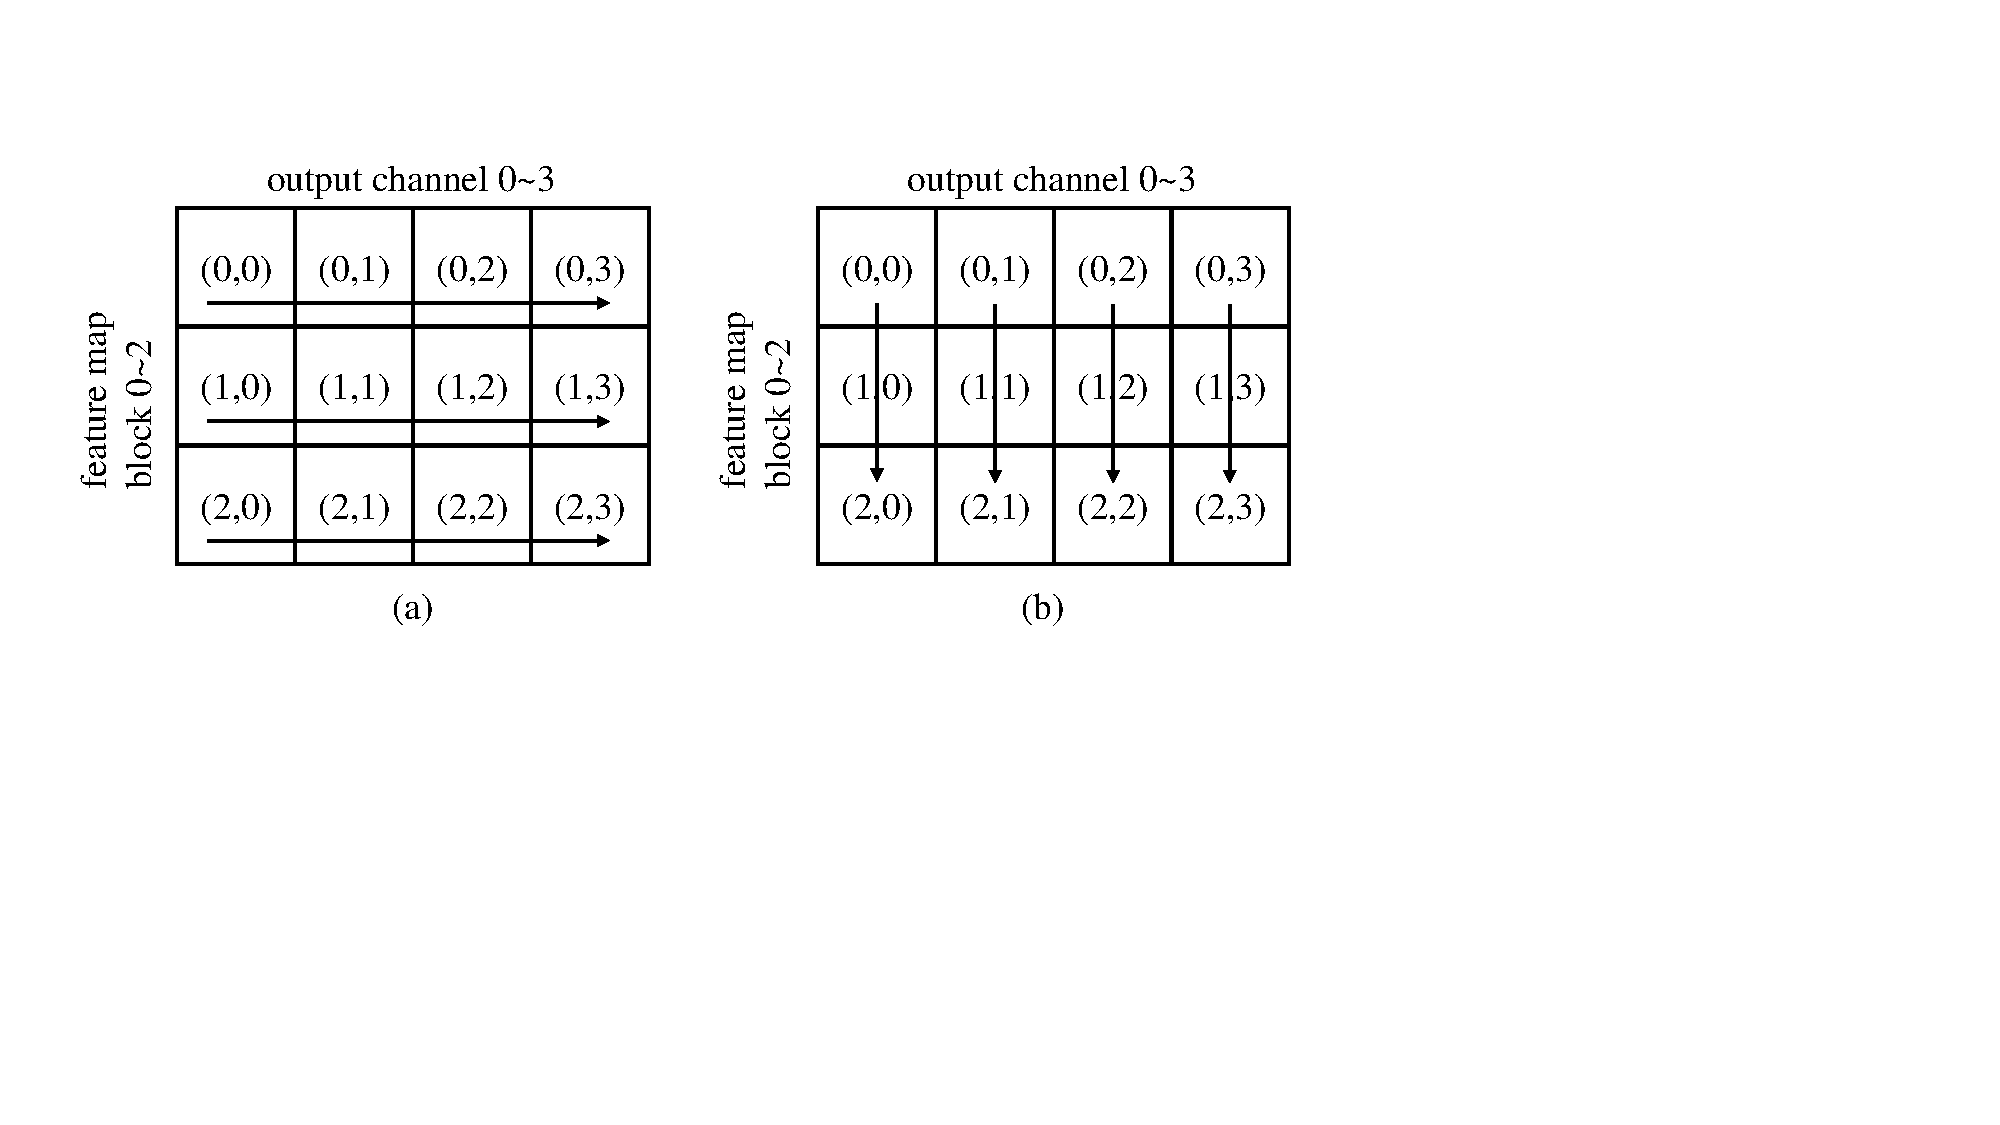
\includegraphics[width=1\columnwidth]{fig/single_layer.pdf}
  \vspace{-20pt}
  \caption{An example of how loop order affects data transfer behavior. Block $(i, j)$ denotes the computation for the $i^{th}$ feature map block on the $j^{th}$ channel. (a) Reuse feature map first and load each weight 3 times. (b) Reuse weight first and load each feature map 4 times.}
  \label{fig:single_layer}
  \vspace{-5pt}
\end{figure}

{\bf{Single Layer Schedule Strategy}.} In the case where on-chip buffer size is smaller than the weight size and feature map size of a single layer, data needs to be loaded multiple times. An example is shown in Figure~\ref{fig:single_layer} where the weight buffer can hold only $1/4$ of the weight and input buffer can hold only $1/3$ of the feature maps. Choosing reuse weights or reuse feature map will cause difference on data transfer behavior and further affects the data transfer energy and data transfer time.

\begin{figure}[t]
  \centering
  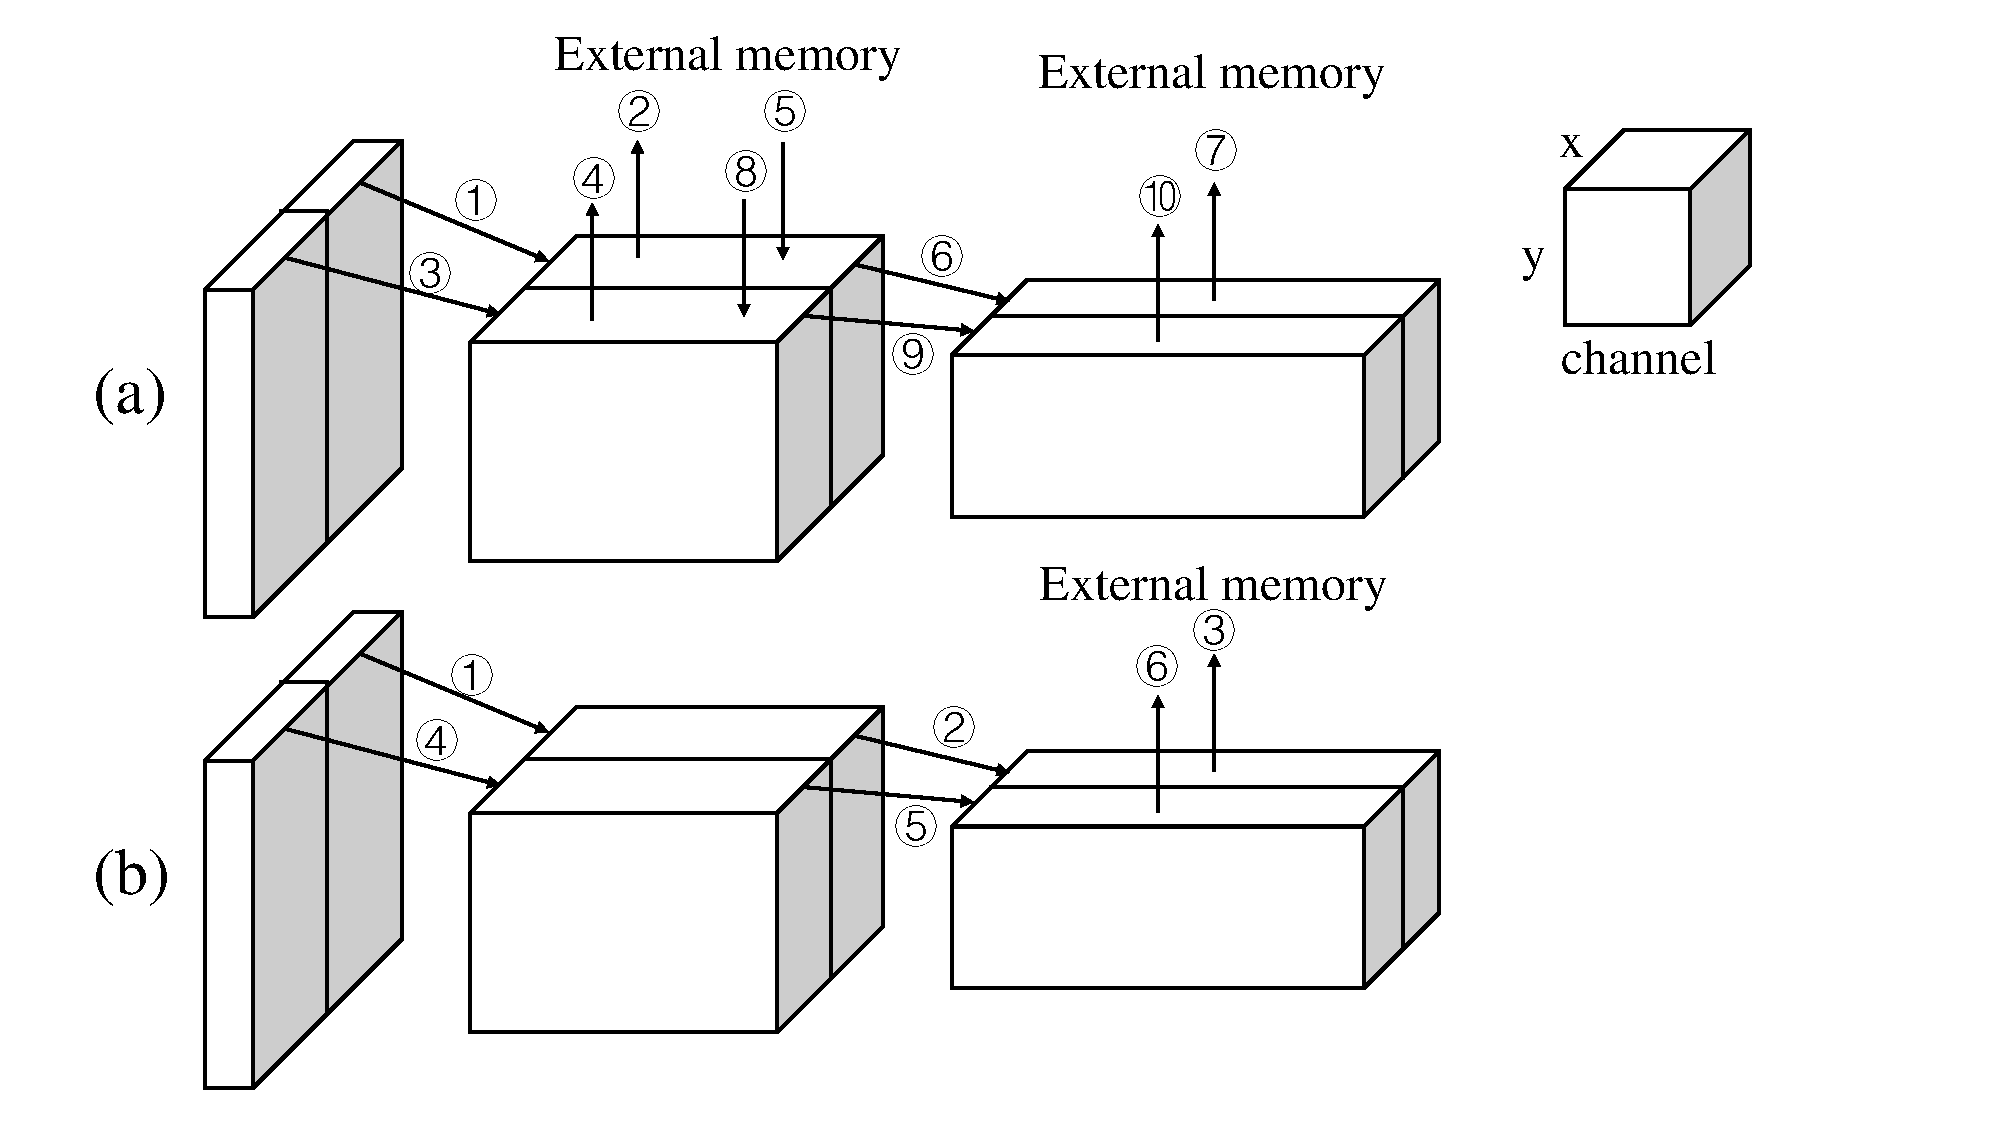
\includegraphics[width=1\columnwidth]{fig/cross_layer.pdf}
  \vspace{-20pt}
  \caption{An example of a cross layer schedule over 3 layers. (a) Single layer schedule. (b) Cross layer schedule.}
  \label{fig:cross_layer}
  \vspace{-5pt}
\end{figure}

{\bf{Cross Layer Schedule Strategy}.} As suggested by~\cite{alwani2016fused}, when the network is processed layer by layer, the result of one layer needs to be written back to external memory it is larger than the output buffer. But if the weight buffer is large enough to contain more than one layers' weight, these layers can be scheduled together to avoid writing the intermediate layers result to external memory. An example is shown in Figure~\ref{fig:cross_layer}, where the cross layer schedule avoids the second layer's feature map to be transferred to and from external memory. As we will implement weight buffer with RRAM, the size of weight buffer can be much larger and thus benefits from this strategy.

{\bf{Fixing Weight On-chip}.} An observation is that if the weight buffer is large enough to hold all the layer's weight on-chip, no weight will need to be read from external memory. With a slightly smaller buffer, we can still follow this idea by fix some of the layer's weights in on-chip buffer to reduce external memory access. So we need to find which layers' weight is to be fixed in the buffer as to minimize the total energy cost.

The solution space of this problem is binary tree of depth $(n+1)$. $n$ denotes the number of CNV layers in the network. To avoid searching the whole $O(2^n)$ solution space, we prune the binary tree with the buffer size limitation. If the the weights on a path already exceeds the weight buffer size, we ignore the search of its subtree. The pseudo code of the optimization process is as follows:

\begin{codebox}
\Procname{\proc{SearchFixedWeight($layers$)}}
\li Let $is\_fixed[1 .. \attrib{layers}{size}]$ be a boolean vector
\li IterSearchFixedWeight($layers, 1, is\_fixed$)
\li \Return $is\_fixed$
\end{codebox}

\begin{codebox}
\Procname{\proc{IterSearchFixedWeight($layers, n, f$)}}
\li \If $l > \attrib{layers}{size}$
\li	\Do
     \Return OptEnergy($layers, f$)
  \End
\li \If available buffer size $< \attrib{layers[n]}{weight\_size}$
\li	\Do
     $f[n] = false$
\li 	\Return IterSearchFixedWeight($layers, n+1, f$)
  \End
\li $f1 = f$; $f1[n] = false$
\li $f2 = f$; $f2[n] = true$
\li $e1 =$ IterSearchFixedWeight($layers, n+1, f1$)
\li $e2 =$ IterSearchFixedWeight($layers, n+1, f2$)
\li $f = (e1 < e2)$ ? $f1$ : $f2$
\li \Return Min(e1, e2)
\end{codebox}